\section{Halbordnungen}
\subsection{Definition}
\begin{frame}
	\begin{Definition}
		Eine Relation $R\subseteq M\times M$ heißt \emph{antisymmetrisch}, wenn für alle $x,y\in M$ gilt $$ xRy \wedge yRx \implies x=y $$
	\end{Definition}
	\pause
	
	\begin{Definition}
		Eine Relation $R\subseteq M\times M$ heißt \emph{Halbordnung}, wenn sie 
		\begin{itemize}
			\item reflexiv
			\item antisymmetrisch
			\item transitiv 
		\end{itemize}
		ist. 
	\end{Definition}

\end{frame}

\subsection{Beispiel}
\begin{frame}
	\emph{Beispiel:} Sei $\sqsubseteq_p$ derart, dass für $v,w\in A^\ast$ gilt: $$ v \sqsubseteq_p w \iff \exists u\in A^\ast : vu = w $$ \pause
	\only<2-3>{Was sagt diese Halbordnung aus? \pause $v\sqsubseteq_p w$ heißt , dass $v$ ein Präfix von $w$ ist. \pause }
	\emph{Beweis}
	\only<4-6>{\begin{itemize}
		\only<4>{\item \emph{Reflexivität}
			$$ v \sqsubseteq_p v \iff \exists u\in A^\ast : vu = v \implies u = \varepsilon $$ Dies ist möglich, da $\varepsilon \in A^\ast$ }
		\only<5>{\item \emph{Antisymmetrie} \begin{align*}
			v\sqsubseteq_p w \wedge w\sqsubseteq_p v &\iff \exists u\in A^\ast : vu = w \wedge \exists \kappa\in A^\ast : w\kappa = v \\ &\implies w\kappa u = w \\ &\implies \kappa = u = \varepsilon \\ &\implies v = w 
		\end{align*}
		}
		\only<6>{ \item \emph{Transitivität}
		\begin{align*}
			v\sqsubseteq_p w \wedge w\sqsubseteq_p x &\iff \exists u\in A^\ast : vu = w \wedge \exists \kappa\in A^\ast : w\kappa = x \\ &\implies vu\kappa = x \\ &\overset{\alpha=u\kappa}{\iff} \exists \alpha\in A^\ast: v\alpha = x \\ &\iff v\sqsubseteq_p x
		\end{align*}
		 }
	\end{itemize}}
\end{frame}

\subsection{Aufgaben}
\begin{frame}
	Zeigen Sie, dass $\leq $ und $\subseteq$ Halbordnungen sind.
\end{frame}
\subsection{Lösung}
\begin{frame}
	Betrachte die Relation $\leq$. Dann gilt mit $$ a\leq b \iff \exists \alpha \in \R^+_0 : a + \alpha = b $$  \pause
	\only<2-4>{
	\begin{itemize}
		\only<2>{\item \emph{Reflexivität}
		\begin{align*}
			a\leq a & \iff \exists \alpha\geq 0 : a + \alpha = a \\ &\implies \alpha = 0 \in \R^+_0
		\end{align*}
		}
		\only<3>{\item
		\emph{Antisymmetrie}
		\begin{align*}
			a \leq b \wedge b \leq a &\iff \exists \alpha, \beta \in\R^+_0 : a + \alpha = b \wedge b + \beta = a \\ &\implies a + \alpha + \beta = a \\ &\overset{\alpha,\beta\geq 0}{\implies} \alpha = \beta = 0 \\ &\implies a = b
		\end{align*}
		}
		\only<4>{\item
		\emph{Transitivität}
		\begin{align*}
			a \leq b \wedge b \leq c &\iff \exists \alpha,\beta \in\R^+_0 : a + \alpha = b \wedge b+\beta = c \\ &\implies a + \alpha + \beta = c \\ &\overset{\gamma=\alpha+\beta}{\implies} \exists \gamma \in\R^+_0 : a + \gamma = c \\ &\implies a\leq c
		\end{align*}
		}
	\end{itemize}	
	}
\end{frame}

\begin{frame}
	Betrachte die Relation $\subseteq$. Dann gilt \pause
	\only<2-9>{
	\begin{itemize}
		\only<2-3>{\item \emph{Reflexivität}
		\begin{align*}
			\only<2>{A \subseteq A &\iff \left( A\subset A \right) \vee \left( A = A \right)}
			\only<3>{A \subseteq A &\iff \left(\textcolor{red}{A\subset A}\right) \vee \left(\textcolor{green}{A = A}\right)}
		\end{align*}
		\only<3>{Dies ist eine wahre Aussage.}
		}
		\only<4-8>{\item
		\emph{Antisymmetrie}
		\begin{align*}
			\only<4-8>{
			A\subseteq B \wedge B\subseteq A \Leftrightarrow & \left( A \subset B \vee A = B \right) \wedge \left( B\subset A \vee B = A \right)
		}
		 \only<5-8>{\\ \Leftrightarrow &  \left( (A\subset B) \wedge \left( B\subset A \vee B = A \right)\right) \\
		 &\vee \left((A = B) \wedge \left( B\subset A \vee B = A \right) \right) \\} 
		\only<6>{\Leftrightarrow &   \left((A\subset B)\wedge (B\subset A) \right) \vee \left( (A\subset B) \wedge (B=A) \right)   \\
		 & \vee  \left( (A=B)\wedge (B\subset A) \right) \vee \left( (A=B) \wedge (B=A) \right)  } 
		\only<7-8>{\Leftrightarrow &   \textcolor{red}{\left((A\subset B)\wedge (B\subset A) \right)} \vee \textcolor{red}{\left( (A\subset B) \wedge (B=A) \right)}   \\
		 & \vee  \textcolor{red}{\left( (A=B)\wedge (B\subset A) \right)} \vee \textcolor{green}{\left( (A=B) \wedge (B=A) \right)}
		 }
		\end{align*}
		}
		\only<8>{Also folgt $$ A\subseteq B \wedge B\subseteq A \implies A = B $$ Dies benutzen wir um Mengengleichheit zu zeigen.
		}
		\only<9>{
		\item
		\emph{Transitivität} 
		\begin{align*}
			A\subseteq B \wedge B\subseteq C &\iff \forall a\in A : a\in B \wedge \forall b\in B : b\in C \\ &\implies a \in C \\ &\implies A\subseteq C
		\end{align*}
		}
	\end{itemize}	
	}
\end{frame}

\subsection{Potenzmengen}
\begin{frame}
	\begin{Definition}
		Als \emph{Potenzmenge} $\mathcal{P}(X)$ ist die Menge aller Teilmengen von $X$ ist definiert. $$ \mathcal{P}(X) = \{ U | U\subseteq X\} $$
		Weitere Notation : $ \mathcal{P}(X) = 2^X $ \\
		
		Für die Mächtigkeit finden wir $$ \vert \mathcal{P}(X) \vert = 2^{\vert X \vert} $$
	\end{Definition} 
	\pause 
	\emph{Beispiel}
	$$ \mathcal{P}(\{a,b\}) = \{ \emptyset, \{a\}, \{b\}, \{a,b\} \} $$
	\pause
	$$\mathcal{P}(\{a,b,c\}) = \{ \emptyset, \{a\}, \{b\}, \{c\}, \{a,b\}, \{a,c\}, \{b,c\}, \{a,b,c\} \} $$
\end{frame}

\begin{frame}
	Betrachten wir nun die Halbordnung $\subseteq$ auf der Menge $\mathcal{P}(\{a,b,c\})$ \pause
	\begin{figure}[H]
		\centering
		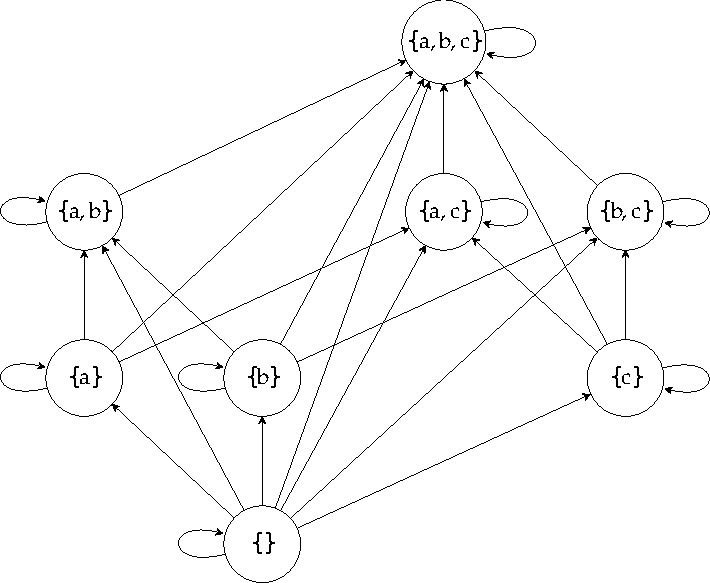
\includegraphics[scale=0.7]{Halbordnung.pdf}
	\end{figure} \pause
	Wird doch recht bald unübersichtlich!
\end{frame}

\section{Hasse-Diagramm}
\begin{frame}
Lassen wir nun einfach die Kanten weg, die sich durch Transitivität und Reflexivität ergeben \pause
\begin{figure}[H]
	\centering
	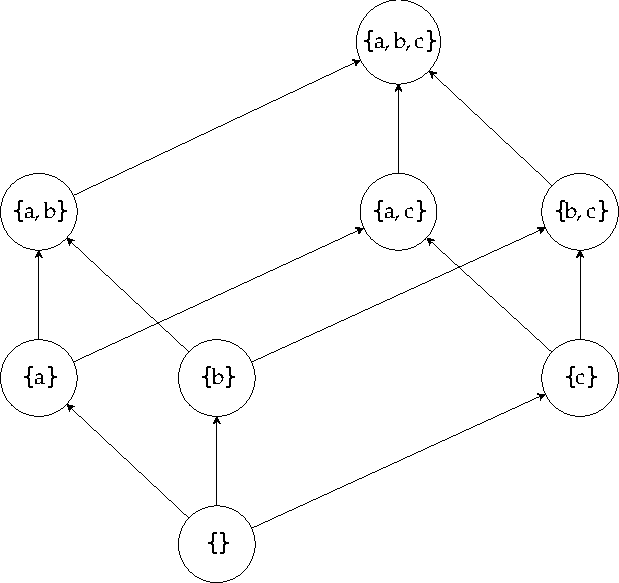
\includegraphics[scale=0.65]{Hasse1.pdf}
\end{figure} \pause
Dies nennen wir das \emph{Hasse-Diagramm}.
\end{frame}

\subsection{Definition}
\begin{frame}
	\begin{Definition}
		Eine Diagramm einer Halbordnung $\sqsubseteq$ auf einer Menge $M$ heißt \emph{Hasse-Diagramm}, wenn es im Diagramm eine Kante gibt von $a$ nach $b$, $a,b\in M$, sofern gilt $$ \nexists c\in M : a\sqsubseteq c \sqsubseteq b $$
	\end{Definition} \pause
	
	\begin{Definition}
		Es sei $(M,\sqsubseteq)$ eine halbgeordnete Menge und $T\subseteq M$. Ein Element $x\in T$ heißt 
		\begin{itemize}
			\item \emph{minimales Element} von $T$, wenn es kein $y\in T, y\neq x$ gibt, mit $y\sqsubseteq x$.
			\item \emph{maximales Element} von $T$, wenn es kein $y\in T, y\neq x$ gibt, mit $x\sqsubseteq y$.
			\item \emph{größtes Element} von $T$, wenn für alle $y\in T$ gilt $y\sqsubseteq x$
			\item \emph{kleinstes Element} von $T$, wenn für alle $y\in T$ gilt $x\sqsubseteq y$
		\end{itemize}
	
	\end{Definition}
\end{frame}

%\begin{frame}
%	Beispiele an der Tafel zu $\sqsubseteq = \subseteq$ und $ M \in \{ \mathcal{P}(\{a\}), \mathcal{P}(\{a\})\cup \{d\}, \{a\}\cup\{d\} \}$
%\end{frame}



\subsection{Aufgabe}
\begin{frame}{WS 10/11}
	Geben Sie das Hasse-Diagramm einer Halbordnung auf einer dreielementigen Menge an, die genau zwei maximale und zwei minimale Elemente besitzt.
\end{frame}
\subsection{Lösung}
\begin{frame}
	\begin{figure}[H]
		\centering
		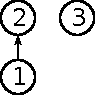
\includegraphics[scale=0.7]{Loesung.pdf}
	\end{figure}
\end{frame}